
%FEHLT: 
% Biogenese eukaryotische RNA
% die 3 lacZ Standardfragen
% Qualitative, Quantitative Bestimmung von Molekülen in Gewebeschnitten
% Bioinformatische Suche nach kodierenden Gen Regionen (genau wie in Musterlösung) = Wie Gen/Expressionsort anhand von Nukleotidsequenz/Proteinsequenz finden, bioinformatisch
% mRNA seq in Prokaryioten die rRNA rausbekommen (genauer)
% MRI: Bauteile & Funktionsweise
% Promotor & Umgebung: Zeichnung beschriften
% Beschriftung DNA <-> RNA -> Protein -> Metabolit
% Enzymfunktion: Alkalische Phosphatase, Endonuklease, Polynukleotidkinase, reverse Transkriptase, Exonuklease, Taq-Polymerase
% Bakterielle rRNA-Anreicherung; tierisches Gewebe -> Genexpression qualitativ und quantitativ bestimmen mithilfe von RNA -> wie gehen Sie vor?
%%%% Relevante Sachen aus dem Praktikum !!
% mRNA-Sequenzierung 
 
\section{Definitionen}

\head{Epigenetik}%3+
Epigenetik ist die Lehre von den \underline{vererbbaren Veränderungen} des Phänotyps, die \underline{nicht mit Veränderungen} \underline{der DNA-Sequenz einhergehen}. \\ \newline 

\head{Nukleotid}%1+
Molekül bestehend aus: 
\begin{itemize}
    \item \underline{Zucker} (Desoxyribose/Ribose)
    \item Eine oder mehrere \underline{Phosphatgruppen}
    \item Eine Stickstoffhaltige \underline{Base}
\end{itemize}$\ $ \\

\head{Lebendtiter}%p+
Die Durchschnittskonzentration der lebenden Zellkolonien \\
Die Konzentration lebender Mikroorganismen, wie Bakterien, Viren oder Hefen, in einer bestimmten Volumeneinheit einer Flüssigkeit. Der Lebendtiter wird normalerweise in koloniebildenden Einheiten pro Milliliter (KBE/ml) oder Plaque-bildenden Einheiten pro Milliliter (PFU/ml) ausgedrückt, abhängig von der Art der Mikroorganismen und der verwendeten Nachweismethode.  \\ \newline

\head{PMF}%10+
"Peptid massen fingerabdruck" (peptid mass fingerprint) \\
Mit hilfe von selektiven Proteasen (bspw. \gls{Trypsin}) und MS können die massen der einzelnen peptide von Proteinen ermittelt werden. Die Summe der Massen entspricht der Proteinmasse. Jedes Protein hat ein einzigartige Masse. \\ \newline

\head{Metabolit}%11+
Ein Zwischenprodukt (Intermediat) in einem meist biochemischen Stoffwechselweg. Bspw. Glukose.  \\ \newline

\head{Nukleosom}%3+
Grundlegende Strukturelle Einheit der Eucaryotischen Chromosomen. Sie bestehen aus einem Komplex aus DNA und Histonen. \\ \newline

\head{Riboswitch}%8+
Ein regulatorisches Segment einer mRNA, das direkt an ein kleines Molekül bindet und dadurch die Expression der kodierten Proteine beeinflusst. \\ \newline

\head{monoklonale und polyklonale Antikörper}
Monoklonale Antikörper sind identische Antikörper, die von einer einzigen Klon von B-Lymphozyten (Plasmazellen) produziert werden. Sie sind spezifisch für ein einziges Epitop auf einem Antigen.\\ Polyklonale Antikörper sind eine Mischung von Antikörpern, die von verschiedenen B-Zell-Klonen produziert werden. Sie erkennen und binden an mehrere Epitope desselben Antigens.  \\ \newline


\head{Operon}%8+
Eine \gls{Transkriptionseinheit} mit Signalen für die RNA-Polymerase, um die Transkription zu starten und zu stoppen. Das Operon kann ein einzelnes Gen (monocistronisch) oder mehrere Gene (polycistronisch) enthalten. Gene werden durch ein polycistronisches Operon gemeinsam reguliert. \index{Operon} \\ \newline

\head{Regulon}%8+
Eine Gruppe von Operons, die sich über das gesamte Genom verteilen, aber von demselben Regulator gesteuert werden. \index{Regulon} \\ \newline

\head{Stimulon}%8+
Die Gesamtheit aller Operons, die auf denselben Stimulus reagieren. \\ \newline

\head{Scaffold}%5
Ein Scaffold ist eine Zusammensetzung von Contigs mithilfe von Paired-End-Bibliotheken. \\ \index{Scaffolding}
\noindent Es besteht aus Contigs und Lücken und kann als eine Art "Gerüst" betrachtet werden, das dazu dient, die Contigs in eine größere, geordnete Struktur zu integrieren.  \\ \newline

\head{Replikon}%2+
DNA- oder RNA-Abschnitt, der ausgehend von einem Replikationsursprung an einem Stück repliziert wird. \\ \newline

\head{Transposon}%3+
Mobile genetische Elemente und können sich von einem Ort im Genom zu einem anderen bewegen, entweder durch einen "Kopieren-und-Einfügen"-Mechanismus oder durch einen "Ausschneiden-und-Einfügen"-Mechanismus. \\ \newline

\head{Disruptionsvektor}
Diese Vektoren sind so konzipiert, dass sie spezifische Gene inaktivieren, um deren Funktion zu untersuchen. Ein Disruptionsvektor enthält typischerweise eine DNA-Sequenz, die homolog zu den Zielbereichen des Gens ist, das inaktiviert werden soll. Diese homologen Sequenzen flankieren ein selektierbares Markergen.  \\ \newline

\head{Synthenie}%6+
Als Syntenie werden in
der Genomik Gemeinsamkeiten in der Reihenfolge von Genen oder Gensegmenten auf verschiedenen chromosomalen Abschnitten beim Vergleich zwischen den Genomen von zwei verschiedenen biologischen Arten bezeichnet. \\ \newline

\head{Genetischer Fingerabdruck}%p+
TODO


\section{Unterschiede}
\head{Unterschied zwischen miRNA und siRNA}%9+
 \underline{miRNAs} regulieren die Genexpression, indem sie an die \glspl{3utr} von Ziel-mRNAs binden und \underline{siRNAs} wirken in der Regel durch die \textit{gezielte Zerschneidung} von komplementären mRNAs.  \\
 Daher können siRNAs auch gezielt gegen fremde RNA verteidigen (Infektion durch ein \gls{RNA-Virus}). \\ \newline

\head{Unterschied Illumina vs. Nanopore}%4+
Der signifikante Unterschied liegt hierbei darin, dass Illumina eine synthetisch
basierte ”short read” Sequenzierung ist. Characteristisch für solche sind ihre
Cluster an vielen kurzen Sequenzen.
Nanopore hingegen ist eine ”long read” Sequenzierung. Dies wird ermöglicht
durch elektronische Spannungsunterschiede bei Nukleotiden in der Nanopore. \\ \newline

\head{Unterschied von BLAST und Smith-(Waterman-Algorithmus?) erklären}%7+
\begin{table}[H]
    \centering
    \begin{tabular}{p{2cm}p{6cm}p{6cm}}
         &  \textbf{BLAST} & \textbf{SMW}\\ \\
       \textbf{Ansatz}  & Heuristisch & Dynamisches Programmieren \\ \\
       \textbf{Empfindlich-keit} & Kann einige optimale Alignments übersehen & Liefert das bestmögliche lokale Alignment 
    \end{tabular}
\end{table}
\noindent Zusammengefasst ist BLAST ideal für schnelle und umfassende Suchen in großen Datenbanken, während der Smith-Waterman-Algorithmus für detaillierte und präzise Analysen geeignet ist, bei denen höchste Genauigkeit erforderlich ist.

\section{Beschreiben und Erklären}

\head{Welche Rolle spielen die Transkriptionsfaktoren bei Operon, Regulon u. Stimulon?}%8+
Transkriptionsfaktoren binden an spezifische DNA-Sequenzen in der Nähe des Promotors eines Operons, um die Transkription der Gene zu regulieren. Sie können entweder als Aktivatoren wirken, die die Bindung der RNA-Polymerase fördern, oder als Repressoren, die die Transkription blockieren. Ein klassisches Beispiel ist das lac-Operon in E. coli, das durch den \underline{lac-Repressor} reguliert wird. \\  \newline Ein \underline{einzelner Transkriptionsfaktor} kann an die Promotorregionen \underline{mehrerer Operons} oder Gene binden, um deren Expression in Reaktion auf bestimmte Signale zu koordinieren. \\ \newline \underline{Mehrere Transkriptionsfaktoren }können beteiligt sein, um die Expression einer Vielzahl von Genen zu koordinieren, die auf den spezifischen \underline{Stimulus} reagieren. \\ \newline

\head{Beschreiben Sie Gen Assembly}
Prozess, bei dem kürzere DNA-Sequenzreads in längere, zusammenhängende Sequenzen oder ganze Genome zusammengefügt werden. \\ \newline

\head{Welche Probleme können bei Gen Assembly auftreten?}
\begin{itemize}
\item \underline{Große Genome}
    \item \underline{Sequenzierungsfehler}: Verschiebung des Leserasters oder schlicht falsche Daten 
    \item \underline{Ungleichmäßige Abdeckung}: bspw. Lücken in der Assemblierung
    \item \underline{Repetitive Sequenzen} sind schwer zu asselmblieren
\end{itemize} $\ $ \\

\head{Wie bestimmt man einen Lebendtiter? (ausführlich)}%p+
\begin{itemize}
    \item Homogenisieren der Probe, um eine gleichmäßige Verteilung der Mikroorganismen zu gewährleisten
    \item Serielle Verdünnungen
    \item Plattieren der Verdünnungen auf Petrischalen mit Nährmedium
    \item Inkubieren der Platten
    \item Koloniezählung
    \item Berechnung des Lebendtiters: 
    \begin{equation*}
        Lebendtiter (KBE/ml) = \frac{\# Kolonien}{Volumen \ der \ Plattierung (ml)} \times Verdünnungsfaktor
    \end{equation*}
\end{itemize} $\ $ \\

\head{Wie erhält man PMF und was stellt es dar?}%10+
PMF stellt die einzigartige Masse von einem Protein dar. Die Ermittlung solcher Masse funktioniert wiefolgt: \\
Das Protein wird in einem SDS-Gel mit selektiven Proteasen verdaut. Das Produkt sind dann die Einzelnen fragmente / peptide des Proteins. Anschließend kann durch \gls{ms} die Masse der einzelnen Peptide ermittelt werden. Die Summe solcher ist dann die Masse des Proteins, welche einzigartig ist. \\ \newline


\head{Prinzip Illuma Sequencing}%4+
Illumina ist eine synthetische basierte ”short read” Sequenzierung mit Clusterbildung ist. Es ermöglicht die parallele Sequenzierung von Millionen von DNA-Fragmenten.
 \\ \newline

\head{Ablauf Illumina}
\begin{itemize}
    \item Extraktion und Fragmentierung der DNA
    \item Hinzufügen von Adaptersequenzen
    \item Cluster-Generierung durch Bridge Amplification und PCR-Amplifikation
    \begin{itemize}
        \item Adaptersequenzen binden sich an Ankerpunkte auf \gls{Flow Cell}
        \item Zugabe fluoreszierender Nukleotide, es wird immer nur eine Base pro PCR-Zyklus hinzugefügt
    \end{itemize}
    \item Anschließende Detektion der Fluoreszenz jedes Clusters
    \item Hinzufügen der nächste Base und Detektion bis Sequenzierung abgeschlossen ist
    \item Bestimmung der Basenabfolge durch Vergleich mit einer Referenzsequenz
\end{itemize}  $\ $ \\

\head{Definieren Sie die Mutationstypen}
\begin{enumerate}
    \item  \textbf{Auxotroph-Mutanten} (Mangel-Mutanten) haben einen Block in einem aufbauenden (anabolischen) Stoff-
wechselweg, der die Synthese eines Zellbausteins (Aminosäure, Vitamin) verhindert. Wachstum kann nur
nach Zusatz des „Bedürfnisses“ zum Medium erfolgen.
\item \textbf{Fermentativ-Mutanten }haben einen Block in einem abbauenden (katabolischen) Stoffwechselweg, wo-
durch die Fähigkeit zur Vergärung einer bestimmten Kohlenstoffquelle (z. B. des Zuckers Lactose) verlo-
ren geht.
\item \textbf{Resistenz-Mutanten} gegen Antibiotika oder Bakteriophagen haben eine Resistenz auf Grund verschie-
dener Mechanismen, wie veränderter Permeabilität der Zellwand, Änderung in der Ribosomenstruktur,
Produktion von Enzymen, die Antibiotika abbauen.
\end{enumerate}
Bzw. auf Sequenz-Ebene (wird nicht gemeint sein...)
\begin{itemize}
    \item \underline{Deletion}: Verlust von Basen 
    \item \underline{Insertion}: Zuästzliche Basen
    \item \underline{Inversionen}: Verdrehung von Basensequenzen um 180°
    \item \underline{bewegliche genetische Elemente}: Insertionen oder unexakt herausgeschnittene Elemente 
    \item \underline{Translokation}: Verlagerung einer Basensequenz 
    \item \underline{Transition}: Eine Pyrimidin-Base wird durch eine anderen Pymiridin-Base ausgetauscht bzw. das selbe mit Purin-Basen
    \item \underline{Transversion}: Purin durch Pyrimidinbase ersetzt oder andersherum 
\end{itemize}  $\ $ \\

\head{Wie schützen sich Bakterien vor fremder DNA?}
Bakterien unterscheiden zwischen eigener und fremder DNA
Fremde DNA wird mithilfe von Restriktionsenzymen abgebaut.
Diesen Prozess bezeichnet man als Restriktion, die abbauenden Enzyme als Restriktionendonukleasen(REN). \\ \newline

\head{Beschreiben Sie die Eigenschaften von Restriktionsendonuklease II}%p+
\begin{itemize}
    \item binden an spezifische DNA-Sequenzen (spezifische Erkennungssequenzen)
    \item schneiden die DNA innerhalb oder in unmittelbarer Nähe der Erkennungssequenz (Präziser und reproduzierbarer Schnitt)
    \item kann \gls{blunt ends} und \gls{sticky ends} erzeugen 
    \item Mg2+-Ionen als Cofaktor, aber keine ATP- oder S-Adenosylmethionin-Cofaktoren (Katalytische Unabhängigkeit)
\end{itemize} $\ $ \\

\head{Welche Eigenschaften muss ein Vektor für tn5 Mutagenese auf jeden Fall aufweisen?}%p+
\begin{itemize}
    \item  die Tn5-Transposon-Sequenz enthalten, einschließlich der invertierten Wiederholungen,
    \item ein Selektionsmarker (meistens Antibiotikaresistenzgen)
    \item Transposase-Gen
    \item Replikationsursprung
    %check
\end{itemize} $\ $ \\


\head{Zu welcher Transposon-Klasse gehört Tn5?}%p+ (muss noch in section rein glaube ich) 
TODO $\ $ \\


\head{Wofür codiert das Lacz-Gen?}
Für $\beta$-Galactosidase \\ \newline

\head{Welchen Nutzen und welche Funktion hat das Lacz-Gen in der Genomik?}
\begin{itemize}
    \item Reportergen in Klonierungsvektoren (Blau-Weiß-Screening)
    \item wird häufig in Klonierungsvektoren integriert, um die erfolgreiche Integration von DNA-Fragmenten zu überprüfen
\end{itemize} $\ $ \\

\head{Wie kann man Metabolite qualitativ u. quantitativ in verschiedenen Regionen untersuchen?}%11+
Qualitativ: Gaschromatographie \\
Quantitativ: Enzymassays \\ \newline

\head{Wie funktioniert qPCR, was ist der Ct-Wert und welche mRNA liegt am meisten vor?}%9+
Methode zur quantitativen Messung von DNA (oder RNA als qRT-PCR). \\ Der Ct-Wert ist der Zyklus, bei dem die fluoreszierende Signale die definierte Schwelle (Threshold) überschreiten und somit deutlich über dem Hintergrundrauschen liegen. \\
Ablauf: 
\begin{itemize}
    \item DNA-Extraktion bzw. extrahierte RNA in cDNA transkribieren 
    \item Amplifikation der (c)DNA
    \item Echtzeit-Detektion der Floreszenz während der PCR-Zyklen 
\end{itemize} 
In einer qPCR-Analyse wird die mRNA mit dem niedrigsten Ct-Wert als die am meisten vorkommende betrachtet. 
\\ \newline

\head{Was ist iPCR? Erkläre das Prinzip.}
\begin{itemize}
    \item \underline{Antigenbindung:} Zielantigen wird an eine feste Oberfläche (z.B. Mikrotiterplatte) gebunden
    \item \underline{Antikörper-DNA-Konjugat:} Zweiter Antikörper, an den ein DNA-Molekül (Molecular Tag) für die Amplifikation gebunden ist, wird hinzugegeben
    \item \underline{Bindung des Konjugats:} Der Antikörper-DNA-Konjugat bindet an das Antigen, das bereits an die Oberfläche gebunden ist und dadurch wird die DNA in der Nähe des Antigens lokalisiert
    \item \underline{PCR-Amplifikation:} Die gebundene DNA wird durch PCR amplifiziert und die Amplifikation der DNA führt zu einer Verstärkung des Signals, das direkt proportional zur Menge des ursprünglichen Zielantigens ist
    \item \underline{Detektion:} Das amplifizierte DNA-Produkt wird mittels standardisierter Techniken wie Gelelektrophorese oder Echtzeit-PCR analysiert, um die Menge des Antigens zu quantifizieren
\end{itemize}  $\ $ \\


\head{Wie funktioniert ein Western Blot?}
Kombi aus Elektrophorese der Immunodetektion zur Detektion spezifischer Proteine in einer Probe. Nutzt SDS-PAGE, Blotting und Antikörper-Inkubation.  \\ \newline


\head{Was ist ein Massenspektrometer/Massenspektrometrie?}%11+
Die Massenspektrometrie (MS) ist eine analytische Methode zur Bestimmung der Masse von Molekülen und ihrer strukturellen Eigenschaften. Ein Massenspektrometer ist das Gerät, das diese Analyse durchführt. \\ \newline

\head{Chromatographie, welche gibt es, welche Eigenschaften müssen die Analyten haben und wie werden sie eluiert?}%11+
\begin{itemize}
    \item \acrlong{hplc}
    \item \acrlong{gc}
    \item \acrlong{lc}
    \item zweidimensionale Gaschromatographie (GC $\times$ GC)
\end{itemize} $\ $ \\
\begin{itemize}
    \item Flüchtigkeit / Löslichkeit 
    \item Unpolarität
    \item Stabilität
\end{itemize}  $\ $ \\
\begin{itemize}
    \item \underline{Gaschromatographie}: Temperaturerhöhung
\end{itemize} $\ $ \\

\head{Metabolitenbestimmung – allgemeiner Ablauf}%11+
\begin{enumerate}
    \item Probengewinnung
    \item Zellaufschluss und Extraktion (Probenvorbereitung)
    \item Derivatisierung
    \item Trennung und Detektion
    \item Generierung der Rohdaten
\end{enumerate} $\ $ \\

\head{Chromosomale DNA-Extraktion - allgemeiner Ablauf}
\begin{itemize}
    \item Probe gewinnen 
    \item Zelllyse
    \item Proteinabbau
    \item Zentrifugation: Entfernung von Zelltrümmern
    \item DNA-Reinigung
    \item DNA-Fällung
    \item Waschen der DNA
\end{itemize} $\ $ \\
\head{Wieso ist BLAST schneller als das Alignment nach W.?}%7+
Weil BLAST heuristisch ist und mit einer definierten Wortgröße, die die Länge der initialen Seed-Segmente bestimmt, arbeitet \\ \newline

\head{Wodurch zeichnen sich bakterielle HFR-Stämme aus?}%2+
\underline{hfr}: DNA effizient von einem Bakterium in ein anderes übertragen (Übertragung vom \gls{fplasmid} und banachbarten Chromosomenregionen) \\
\underline{Integriertes Plasmid}: \gls{fplasmid} (Fertility-Plasmid) ist in das Chromosom eines Bakteriums integriert  \\ \newline

\head{Wie entstehen bakterielle HFR-Stämme?}%2+
Indem ein \gls{fplasmid} (Fertility-Plasmid) durch homologe Rekombination in das Chromosom eines Bakteriums integriert wird. \\ \newline

\head{Worin unterscheiden sich unterschiedliche HFR-Stämme?}%2+
In der Position der Integration des \gls{fplasmid}s und den Genen des integrierten \gls{fplasmid}s und somit den daraus resultierenden Eigenschaften.\\ \newline

\head{Wofür werden HFR-Stämme verwendet?}%2+
In der Mikrobiologie und Genetik, um Gene zu kartieren und die Geninteraktionen innerhalb von Bakterien zu untersuchen. \\ \newline

\head{Was ist MALDI-Imaging und was wird damit dargestellt?}%11+
Massenspektrometrie Methode um die Verteilung von Molekülen in einem Gewebeschnitt darzustellen. \\ \newline

\head{Was ist Southern Blot? Erkläre das Prinzip.}%3+
Schneller Nachweis einer Gensequenz in einem Genom durch das Übertragen der durch Gelelektrophorese aufgetrennten DNA-Fragmente auf eine Membran und anschließender Hybridisierung der Ziel-Sequenzen mit markierten Sonden.  \\ \newline

\head{Was sind die Vorteile langer Reads?}%4+
Direktes Lesen von epigenetischen Modifikationen und direkte Sequenzierung einzelner DNA-Moleküle. \\ \newline

\head{Was sind die Nachteile von Oxford Nanopore?}%4+
Hohe Fehlerrate und Anschaffungskosten sehr hoch. \\ \newline

\head{Erklären sie die wichtigsten bestandteile von Souther Hybridisierung}%3+
\begin{enumerate}
    \item DNA-Extraktion und -Aufbereitung (Reinigung)
    \item Restriktionsenzym-Verdau
    \item Gelelektrophorese
    \item Denaturierung
    \item Transfer auf eine Membran
    \item Hybridisierung mit einer markierten Sonde
    \item Waschen
    \item Detektieren
\end{enumerate}
Bestandteile: Papiertücher, Nylonmenbran, Gel Puffer, Support, Schnur, Kammer \\ \newline


\head{Was ist PACBIO-SMRT-Sequencing?}%4+
Eine Single-Molecule Sequencing-Methode, die Sequenzierung in Echtzeit und ohne vorherige Amplifikation ermöglicht.  \\
Während die DNA-Polymerase die DNA repliziert, werden fluoreszenzmarkierte Nukleotide eingebaut. Die Fluoreszenzfarbstoffe befinden sich an den Phosphatgruppen der Nukleotide. Sobald ein Nukleotid eingebaut ist, wird der Farbstoff abgespalten und erzeugt ein Fluoreszenzsignal. \\ \newline


\head{Eigenschaften für Vektoren mit large-insert Klonen. Nennen sie zwei Beispiele.}%5+
\begin{itemize}
    \item Hohe Kapazität (bp)
    \item Origin of replication
    \item Stabilität
\end{itemize}
BAC / YAC \\ \newline

\head{Welcher Schritt ist ausschlaggebend für die Pyrosequenzierung? In welchem Schritt wird detektiert?}%4+
Wenn die DNA-Polymerase ein Nukleotid einbaut, so wird Pyrophosphat (PPi) freigesetzt.\\
Solches ist entscheident, da es durch die Enzyme ATP-Sulfurylase und Luciferase in Lichtsignale umgewandelt wird. \\
Das Detektieren passiert ganz am Ende, indem eine Kamera die Lichtsignale aufzeichnet. \\ \newline


\head{Beschreiben sie die Isolierung von Plasmid-DNA}%2+
\begin{enumerate}
    \item Kultivierung der Bakterien
    \item Ernte der Zellen und Lyse
    \item Neutralisation: Fällung von Zelltrümmern, Proteinen und chromosomaler DNA
    \item Zentrifugation
    \item Reinigung der Plasmid-DNA
    \item Fällung der Plasmid-DNA
    \item Waschen des DNA-Pellets
\end{enumerate}

\head{Ablauf einer Klonierung}%2+
\begin{itemize}
    \item DNA und \gls{vektor}-DNA isolieren \index{Vektor}
    \item DNAs mit Restriktionsenzymen\index{Restriktionsenzym} schneiden
    \item Isolierte DNA und \gls{vektor}-DNA kombinieren und ligieren
    \item Transformation\index{Transformation} in Bakterien 
    \item Bakterien kultivieren
\end{itemize}  $\ $ \\

\head{Was ist ein SuicidePlasmid und wofür wird es verwendet?}
Suicide-Plasmide sind Plasmide, welche in einem bestimmten Wirtsbakterium nicht repliziert werden können.
Sie werden eingesetzt für gezielte Mutationen bei Bakterien. \index{Suicide-Plasmid}  
\\ \newline

\head{Wie ist der Ablauf von Sanger Sequencing?}%4+
\begin{enumerate}
    \item 1. Primer bindet and 5’ ende des komplementären Stranges und wird mit
einer DNA Polymerase verlängert.
\item 2. Es werden dann Desoxynukleotide (dNTP) bis zur vorletzten Position
angehängt.
dNTP’s sind: dATP, dCTP, dGTP, dTTP
\item 3. Das letzte Nukleotid ist ein Didesoxnukleotid (ddNTP). Da solches keine OH Gruppe am 3’ Ende besitzt können keine weiteren Nukleotide angehangen werden. Somit ist dann die Sequenzierung zuende! ddNTP’s sind: ddATP, ddCTP, ddGTP, ddTTP
\end{enumerate} $\ $ \\

\head{Prinzip der Sanger Sequenzierung und seiner Nachweis- u. Detektionsmethoden?}%4+
Kettenabbruchmethode: Während der DNA-Synthese durch die DNA-Polymerase werden die ddNTPs in die wachsende DNA-Kette eingebaut. Wenn ein ddNTP eingebaut wird, stoppt die Verlängerung der DNA-Kette, da keine weitere Bindung möglich ist. \\ Dieser Prozess führt zu einer Mischung von DNA-Fragmenten unterschiedlicher Länge, die jeweils mit einem ddNTP enden. Jedes ddNTP ist typischerweise mit einem einzigartigen Fluoreszenzfarbstoff markiert. \\ \newline

\head{Wichtige Komponenten und Enzyme der Sanger-Sequenzierung}%4+
\begin{itemize}
    \item \glspl{dntp}
    \item \glspl{ddntp}
    \item DNA-\gls{Polymerase}
    \item Pufferlösung
    \item Fluoreszenzfarbstoffe
\end{itemize} $\ $ \\

\head{Beschreiben Sie die Umsetzung der genetischen Information in Eukaryoten unter Benennung der relevanten Zwischenstufen.}%1+
\begin{enumerate}
    \item Nukleus: Transkription
    \item Nukleus: Bildung der pre-mRNA durch Anfügen eines CAPs am 5' Ende.
    \item Nukleus: Bildung der polyadenylated
pre-mRNA durch Anfügen einer poly A Kette am 3' Ende.
    \item Nukleus: Bildung der mRNA durch splicing.
    \item Cytoplasma: Translation der mRNA
    \item ER und Golgi-Apparat: Faltung der RNA in die unterschiedlichen Strukturen bis zum finalen Protein.
\end{enumerate} $\ $ \\

\head{Wie funktioniert Northern Blot? Und wofür wird es verwendet?}%9+
\begin{enumerate}
    \item RNA-Extraktion und -Aufbereitung (Reinigung)
    \item Gelelektrophorese
    \item Transfer auf eine Membran
    \item Hybridisierung mit einer markierten Sonde
    \item Waschen
    \item Detektieren
\end{enumerate} $\ $ \\

\head{Durch einen Sequenzierfehler wurde eine zusätzliche Base in die Sequenz eingebaut. Welche späteren Folgen kann dies haben?}%4+
Durch die Insertion wurde das Leseraster der Basentrippletts verändert. Somit kann es zu missinterpretationen der Proteinsequenzen und oder zu falschen bzw. keinen Ergebnissen in dem Datenbank abgleich führen. \\ \newline

\head{Nennen Sie drei verschiedene Inonisierungsmethoden}%11+
\begin{itemize}
    \item Elektrospray-Ionisation (ESI) 
    \item MALDI
    \item Elektronenstoß-Ionisation (EI)
\end{itemize} $\ $ \\

\head{Sie wollen die Genexpression in einer prokaryotischen Zelle quantitativ und qualitativ messen. Wie gehen Sie vor?}%9+
Als Qualitative Analyse führt man eine RT-PCR durch, um herauszufinden, ob ein Gen in der Probe exprimiert wird. \\
Als quantitative Analyse führt man eine qPCR mit anschließender RNAseq durch  \\ 
Man kann auch direkt eine RT-qPCR durchführen und anschließend eine RNAseq.  \\ \newline

\head{Bennen Sie die wesentlichen Eigenschaften eines BAC-Vektors}%5+
\begin{itemize}
    \item große Kapazität
    \item hat Replikationsursprung
    \item hat Selektionsmarker
    \item Stabile Vererbung
    \item MCS
\end{itemize} $\ $ \\

\head{Wofür setzt man einen BAC-Vektor ein?}%5+
\begin{itemize}
    \item Klonierung großer DNA-Fragmente
    \begin{itemize}
        \item Genomkartierung
        \item Sequenzierung
        \item Studien zur genetischen Variation
    \end{itemize}
\end{itemize} $\ $ \\

\head{Wofür steht SDS-Page? Was wird damit gemacht?}%2+
\gls{sds} steht für Sodium Dodecylsulfat-Polyacrylamidgelelektrophorese und ist eine Methode um Proteine nach Masse zu trennen. Es wird bei der 2D Gelelektrophorese als zweite Dimension verwendet. \\ \newline

\head{Siewollen ein unbekanntes prokaryotisches Gen für einen Stoffwechsel identifizieren. Wie gehen Sie vor?}
\texttt{Noch machen} %TODO 
\\ \newline

\head{Erklären Sie die Begriffe Ortholog, Paralog und Homolog}%6+
\begin{itemize}
    \item homolog: Zwei Gene (oder Proteine) sind zueinander homolog, wenn sie von einem gemeinsamen Vorläufer abstammen.
Meist basieren Homologie-Zuweisungen auf Ähnlichkeiten in Sequenz oder Struktur
\item ortholog: homologe Gene, die in verschiedenen Organismen vorkommen und auf einen gemeinsamen Vorfahren
zurückgehen, der vor der Aufspaltung der Art existierte. Orthologe Gene haben in der Regel die gleichen oder sehr ähnliche Funktionen.
\item paralog: homologe Gene, die durch ein Duplikationsereignis im Genom entstanden sind. Es handelt sich um neue Gene, die neue (häufig dem Ursprungsgen noch ähnliche) Funktionen kodieren. Paraloge Gene befinden sich häufig im selben Genom
\end{itemize} $\ $ \\

\head{Was macht X-Gal?}%5+
Enzym; Kann von $\beta$-Galactosidase gespalten werden und daraus entsteht ein blauer Farbstoff. So kann man $\beta$-Galactosidase nachweisen. (Blau-Weiß-Screening) \\ \newline

\head{Was versteht man unter dem Begriff RNAseq?}%9+
RNA-Sequenzierung - quantitative Methode zur Analyse des Transkriptoms eines Organismus. \\ \newline

\head{Erläutern Sie das Prinzip der RNAseq und skizzieren Sie den Workflow}%9+
Prinzip: RNA-Moleküle in cDNA umzuschreiben und diese dann zu sequenzieren  \\
Workflow: 
\begin{enumerate}
    \item RNA Isolierung
    \item (RNA Fragmentierung)
    \item cDNA Synthese
    \item Sequenzierung
    \item (weitere Analyse)
\end{enumerate} $\ $ \\

\head{Wie viele Genome gibt es in einem typischen Prokaryoten?}%2+
Ein Bakterium wäre ein typischer Prokaryot. Bakterien haben typischerweise ein Chromosom als Hauptgenom und das Plasmidgenom.  \\ \newline

\head{Wie funktioniert eine Gaschromatographie?}%11+
\begin{itemize}
    \item Metabolite müssen derivatisiert werden.
    \item Mit Trägergas (mobiler Phase) durch Kapillarröhre (Säule) gedrückt.
    \item Säule ist mit stationärer Phase ausgekleidet.
    \item Je nach Polarität und Dampfdruck verweilen Metabolite unterschiedlich lang in der stationären Phase.
    \item Zeit in der Säule wird gemessen.
    \item Mit Standard vergleichen.
\end{itemize} $\ $ \\

\head{Wofür verwendet man Gaschromatographie?}%11+
Zur Auftrennung von Metabolitgemischen. \\ \newline

\head{Wofür ist das Produkt des Lacz-Gens verantwortlich? }
$\beta$-Galactosidase hat zentrale Rolle im Laktosestoffwechsel von Bakterien: 
Hydrolyse von Laktose in Glukose und Galaktose oder Isomerisierung in Allolactose; Regulation des lac-Operons über Allolactose \\ \newline

\head{Wofür wird das LacZ in der Gentechnik verwendet?}
Reportergen und als Werkzeug zur Selektion und Identifizierung von rekombinanten Klonen verwendet. \\ \newline

\head{Plasmid Isolierung- Wie heißt dieser Vorgang?}%5+
Miniprep \\ \newline

\head{Coding Sequenz bioinformatisch analysieren - wie geht das?}%7+
\begin{itemize}
    \item Festlegung der minmalen ORF-Länge 
\item Suche nach Stopp
\item Suche Stromaufwärts nach entferntesten Start
\item Scanning in allen 6 Leserastern
\end{itemize}
Andere Methoden:
Codon Usage, Homologiesuche \\ \newline

\head{Erklären Sie Whole Shotgun und Ordered Shotgun}%5+
\begin{itemize}
    \item \underline{WGS}: Bei WGS wird das gesamte Genom in viele kleine, zufällige Fragmente zerlegt. Diese Fragmente werden dann sequenziert, ohne dass eine vorherige physische Kartierung des Genoms erfolgt.
    \begin{itemize}
        \item Die DNA wird fragmentiert und die Fragmente werden in Vektoren kloniert oder direkt sequenziert.
        \item Die resultierenden Sequenzdaten werden mithilfe von Computerprogrammen zur Überlappung analysiert und zu einem vollständigen Genom zusammengesetzt.
    \end{itemize}
    \item \underline{OGS}: OGS ist ein systematischerer Ansatz, bei dem das Genom zuerst in geordnete Segmente unterteilt wird, bevor die einzelnen Fragmente sequenziert werden.
    \begin{itemize}
        \item Zunächst wird eine physische Karte des Genoms erstellt, indem große DNA-Fragmente (z.B. in BACs oder YACs) geordnet und kartiert werden.
        \item Diese großen Fragmente werden dann in kleinere Stücke zerlegt, und jedes wird separat sequenziert.
        \item Die Sequenzen werden mithilfe der physischen Karte und der bekannten Anordnung der großen Fragmente zusammengesetzt.
    \end{itemize}
\end{itemize} $\ $ \\ 

\head{Welches Genom gibt es nur in Pflanzenzellen?}%3+
Plastom \\ \newline

\head{Was weißt auf den prokaryotischen Ursprung einiger dieser Genome hin?}%3+
Organellengenome weisen Merkmale auf, die an prokaryotische Genome erinnern (Endosymbiontentheorie). \\
Genomische Analysen zeigen, dass viele Gene in Mitochondrien und Chloroplasten eine enge Verwandtschaft mit Genen von bestimmten Gruppen von Bakterien aufweisen, wie Alphaproteobakterien im Fall von Mitochondrien und Cyanobakterien im Fall von Chloroplasten. \\ \newline

%\head{In Bakterien gibt es RNA-Schalter, die als Temperatur-Schalter funktionieren. Erklären Sie das Prinzip.}
%\head{In welchen Bakterien findet sich so ein Temperatur-Schalter?}

%\head{Wie kann man das 5'-Ende (das erste Nukleotid) einer mRNA in Bakterien identifizieren?}

%\head{In Bakterien gibt es RNA-Schalter, die auf Metabolite reagieren. Erklären Sie das Prinzip der regulation (was wird reguliert!). Beschreiben und benennen Sie den Bindungsmodus dieser RNA-Schalter und Matabolite!}
%\head{In welchen Bakterien findet sich so ein Metabolit-sensitiver Schalter?}

\head{Wie kann man eine Restriktionsschnittstelle kartieren ohne Sequenzierung und mit Hilfe anderer Restriktions Fragmentlängen?}
TODO 

\head{Wie ist der Ablauf zur Gewinnung eines genetischen Fingerabdrucks?}%p+
TODO
\head{Was sind die Eigenschaften von Restriktionsenzyme der Klasse II?}%p+
TODO

\section{Beschriften und zeichnen}

\head{Kodierendes Eukaryonten Gen beschriften}%3+
\begin{figure}[H]
    \centering
    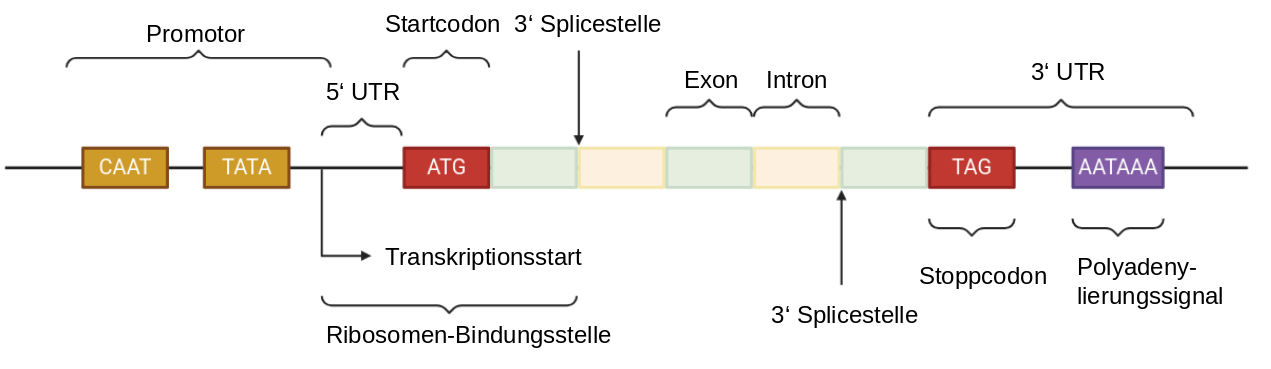
\includegraphics[width=12cm]{images/eukgenfilled.png}
\end{figure}

\head{Skizzieren sie einen BAC-Vektor}%5+
\begin{figure}[H]
    \centering
    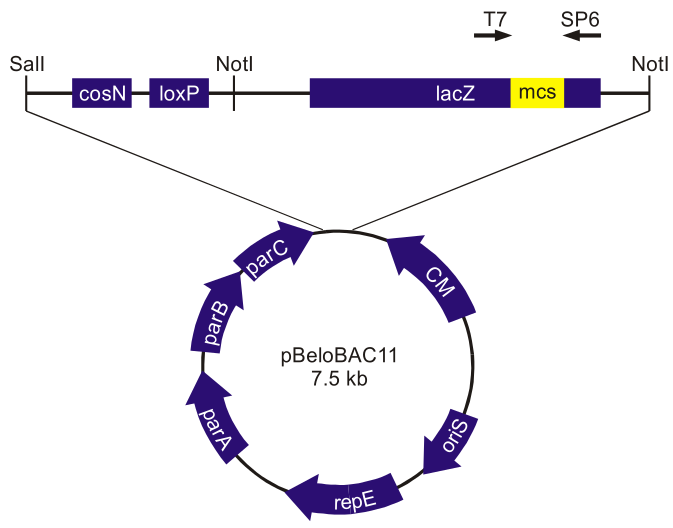
\includegraphics[width=10cm]{images/bacvector.png}
    \caption{\underline{BAC-Vektor}: \textit{parA, parB, parC}: Aufteilung (partitioning) auf Tochterzellen während Zellteilung, stabile Weitergabe;  \textit{\gls{repe}}; \textit{CM}: Antibiotikaresistenz (Chloramphenicol)}
    \label{fig:bacvector}
\end{figure}

\head{Zeichnen Sie das tn5 Transposon (detailliert)}%p+
\begin{figure}[H]
    \centering
    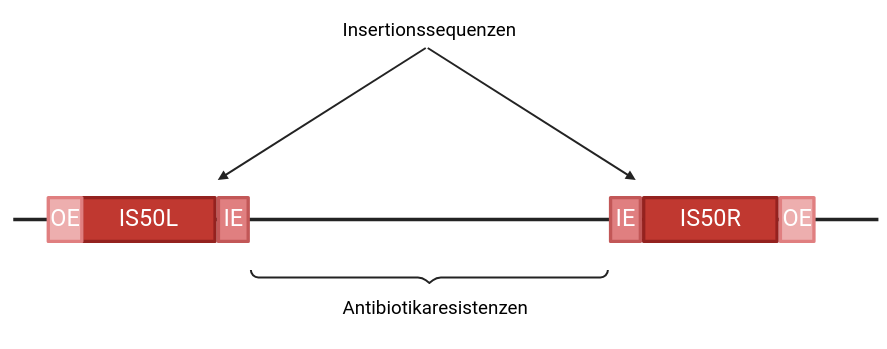
\includegraphics[width=12cm]{images/tn5.png}
\end{figure}
\head{Beschriften eines Antikörpers}
TODO 
\head{Blunt und sticky ends einzeichnen}
TODO 
\head{Skizzieren Sie den Ablauf eines Proteinversuchs von der Zellkultur bis zur Auswertung}
\begin{figure}[H]
    \centering
    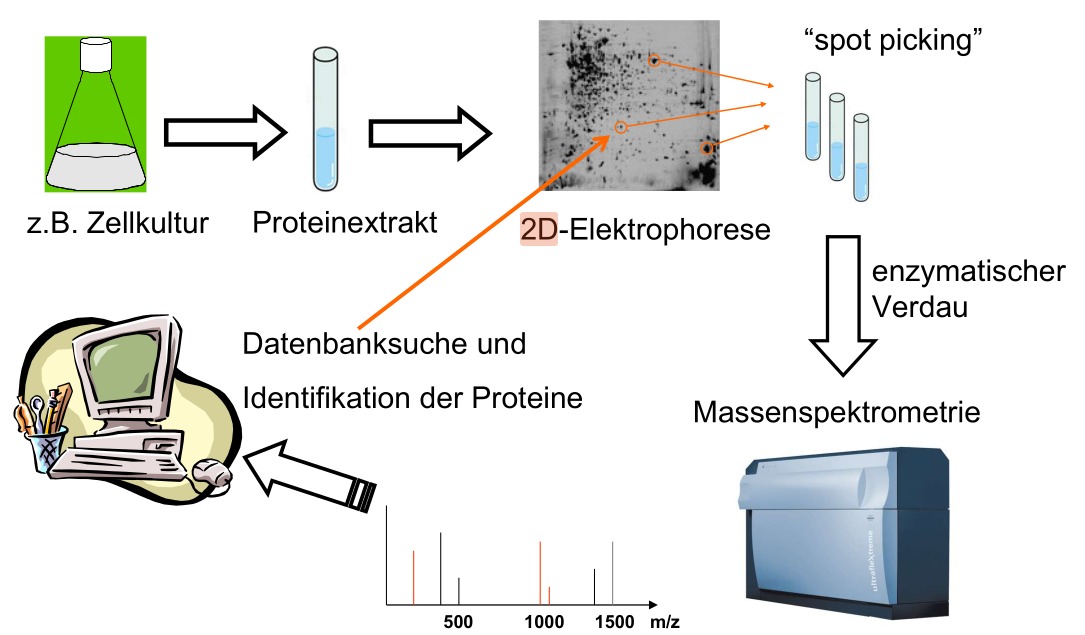
\includegraphics[width=12cm]{images/proteinversuch.png}
\end{figure}

\testhead{Zeichne ein IS-Element}%p+
TODO

\section{Multiple Choice}
\head{Was ist der Tanspositionsmechanismus von Tn5? (1 Antowort)}%p+
TODO
\begin{itemize}
    \item[[ ]] □ konservativ
\item[[ ]] □ multiplikativ
\item[[ ]] □ transpositiv
\item[[ ]] □ replikativ
\end{itemize}
\head{Welche der folgenden Eigenschaften hat ein suicide-Vektor}%p+
TODO
\begin{itemize}
    \item[[ ]] □ Transposon
    \item[[ ]] □ Breiter Wirtsbereich
    \item[[ ]] □ IS-Element
    \item[[ ]] □ Eingeschr¨ankter Wirtsbereich
    \item[[ ]] □ Mutator
    \item[[ ]] □ oriT
\end{itemize}
\head{Welche der folgenden Eigenschaften hat ein IS-Element}%p+
TODO
\begin{itemize}
    \item[[ ]] □ suicide
    \item[[ ]] □ IR
    \item[[ ]] □ Replikase
    \item[[ ]] □ Transponase
    \item[[ ]] □ broad host range
    \item[[ ]] □ repeats
\end{itemize}v

\section{Beispiele}
\head{3 Beispiele von epigenetischen Modifikationen an Histonen}%3+
\begin{itemize}
    \item Acetylierung
    \item Methylierung
    \item Ubiquitinierung von Lysin
    \item Phosphorylierung von Serin- und ThreoninrestenF
\end{itemize} $\ $ \\

\head{3 NAPs}%3+
\begin{itemize}
    \item HU
    \item H-NS
    \item Fis
    \item IHF
\end{itemize} $\ $ \\

\head{Nenne Sie drei verschiedene Inonisierungsmethoden}%11+
\begin{itemize}
    \item Elektrospray-Ionisation (ESI) 
    \item MALDI
    \item Elektronenstoß-Ionisation (EI)
\end{itemize} $\ $ \\

\head{Bennen Sie die drei (Sub)Genome einer eukaryotischen Zelle}%3+
\begin{itemize}
    \item Nukleom: Kern-Genom \index{Nukleom}
    \item Chondriom: Mitochondrium-Genom (variabel in Größe und Struktur) \index{Chondriom}
    \item Plastom: Chloroplasten-Genom (gleichbleibende allgemeine Struktur) \index{Plastom}
\end{itemize} $\ $ \\

\head{3 Techniken, um Genexpression zu messen/untersuchen}%9+
\begin{itemize}
    \item qRT-PCR
    \item RNA-Seq
    \item Microarray-Analyse
    \item Nothern Blotting
\end{itemize} $\ $ \\

\head{Bestandteile des Massenspektrometers}%11+
\begin{itemize}
    \item Ionenquelle
    \item Massenanalysator
    \item Detektor
\end{itemize} $\ $ \\

\head{Reaktionskomponenten der PCR und deren ungefähre Temperaturen}
\begin{itemize}
    \item Denaturierung (~94°)
    \item Annealing (~50–65°C) - Primer 
    \item Elongation (~72°C)  - DNA-Polymerase
\end{itemize} $\ $ \\

\head{Nennen Sie die drei wichtigsten Komponenten der Klonierung und ihre Funktion.}%2+
\begin{itemize}
    \item \gls{vektor} – überträgt DNA
    \item \gls{sds}\index{SDS-Page} – Darstellung
    \item \gls{gfp} – Marker \index{GFP}
\end{itemize} $\ $ \\

\head{Nennen sie zwei Beispiele für large insert clone Vektoren}%5+
\begin{itemize}
    \item BAC
    \item YAC
\end{itemize} $\ $ \\

\head{3 versch. Techniken zum Messen des Expressionszustand von Genen + deren wesentliche Eigenschaften}%9
\begin{itemize}
    \item qRT-PCR
    \item RNA-Seq
    \item Microarray-Analyse
    \item Nothern Blotting
\end{itemize} $\ $ \\


\begin{figure}[H]
    \centering
    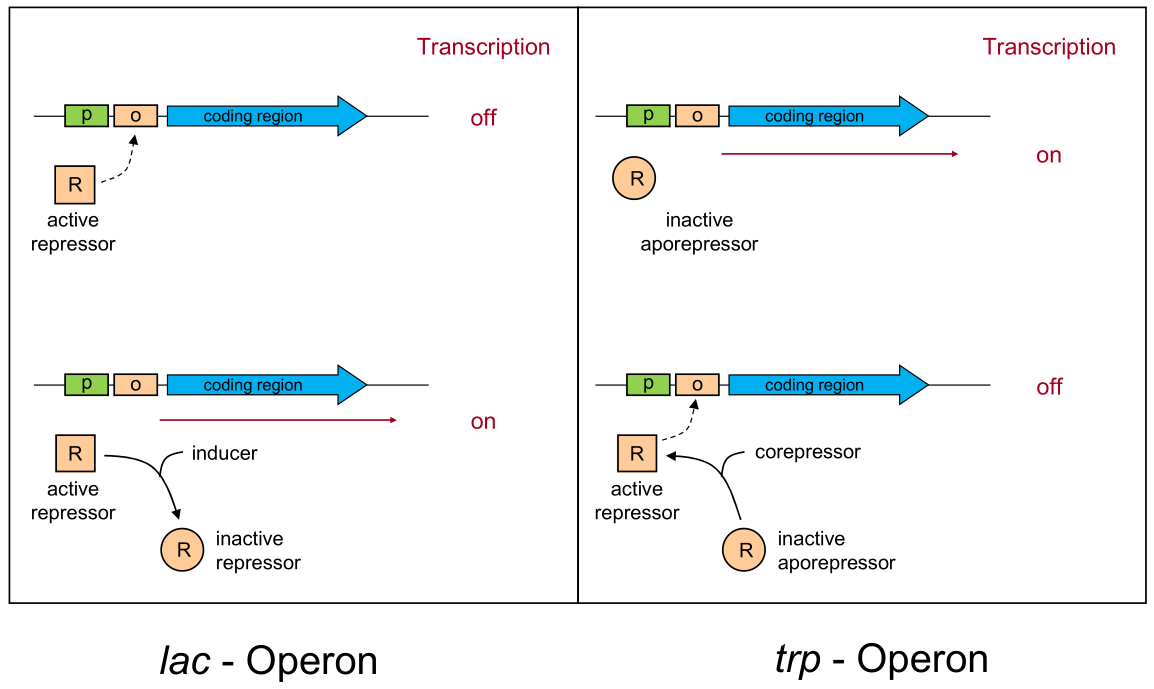
\includegraphics[width=12cm]{images/repressorbildfilled.png}
\end{figure}

